\documentclass[12pt]{article}

\pagestyle{empty}
\setcounter{secnumdepth}{2}

\topmargin=0cm
\oddsidemargin=0cm
\textheight=22.0cm
\textwidth=16cm
\parindent=0cm
\parskip=0.15cm
\topskip=0truecm
\raggedbottom
\abovedisplayskip=3mm
\belowdisplayskip=3mm
\abovedisplayshortskip=0mm
\belowdisplayshortskip=2mm
\normalbaselineskip=12pt
\normalbaselines

\usepackage{graphicx}
\usepackage{float}
\usepackage{titlesec}
\usepackage{pdflscape}

\setcounter{secnumdepth}{3}
\pagenumbering{arabic}
\pagestyle{plain}

\begin{document}

\vspace*{0.5in}
\centerline{\bf\Large Test Document}

\vspace*{0.5in}
\centerline{\bf\Large Team PB-PI}

\vspace*{0.5in}
\centerline{\bf\Large April 8, 2018}

\vspace*{1.5in}
\begin{table}[htbp]
\caption{Team}
\begin{center}
\begin{tabular}{|r | c|}
\hline
Name & ID Number \\
\hline\hline
Alissa Bellerose & 27377320 \\
Sabrina D'Mello & 27739486 \\
Melanie Damilig & 40032420 \\
Tobi Decary-Larocque & 27407645 \\
Zain Farookhi & 26390684 \\
Giulia Gaudio & 27191766 \\
Jason Kalec & 40009464 \\
Damian Kazior & 40016168 \\
Johnny Mak & 40002140 \\
Philip Michael & 40004861 \\
Ramez Nicolas Nahas & 26718108 \\
Steven Tucci & 40006014 \\
Shunyu Wang & 40043915 \\
\hline
\end{tabular}
\end{center}
\end{table}

\clearpage

\section{Introduction}

This document contains the overall test plan for the myMoney application. The myMoney application is a tool for young adults and students to keep track of their spending and help with their budgeting. This test plan describes the different tests performed to ensure a working program and explains the reasoning for the tests.\\

The purpose of this document is to provide assurance and show the reliability of the software. The test plan therefore includes:

\begin{itemize}
  \item An overall view of the different tests performed
  \item A description of the tests
  \item References to the use cases and requirements satisfied by testing
\end{itemize}

Testing the program's different functionalities involves different types of tests. Unit, integration and user interface testing were performed for the purpose of this document. This was managed via black-box, white-box and boundary testing.

\section{Test Plan}

For the deposit and withdraw use cases, different unit tests were performed (including boundary tests) to ensure functionality. The different test cases were designed to test each part of each use case. This includes the format of what the user inputs, as well as ensuring that the database is updated or not, according to whether the transaction is legal or not.\\

In regards to our requirements document, the test plan references the deposit and withdrawal use cases specifically. The tests for each of these use cases are integral to the proper functionality of the application and are therefore an important part of the testing sequence. The balance display use case does not have any functional testing to ensure that it works correctly, but any modification to the user's balance should be reflected through the appropriate view. Similarly, the use cases for the ``Show History'' functionality as well as "Export History" do not rely on any user input except for a button click, so testing was only performed to make sure the output files are correct.\\

There were no tests performed to check if the application is portable to all operating systems described in the non-functional requirements, since the application is not being exported as a stand-alone app. It will function within the Eclipse environment for the time being.

\subsection{System Level Test Cases}

\subsubsection{Deposit Test Case} \label{tc:1}

\noindent
{\bf Purpose}\\
If the amount provided by the user is valid (a positive number), the ``deposit money'' functionality should add the amount indicated by the user to the account (database) and increment the ``Current Balance'' field by the amount indicated.  If the user provided an invalid amount, such as a string or a negative number, the system should display an error message and not update the account (database) and ``Current Balance''.  The purpose of the Deposit Test Case is the following: verify that the deposit money functionality works as described above.

\noindent
{\bf Input Specification (see Figure 3 and Figure 4)}

\paragraph{1.1. ``Amount'' input text field}
\subparagraph{Purpose} The user enters the amount to deposit in the ``Amount'' input text field.

\subparagraph{Test Data} Requirement: This amount should be a positive number (decimal or integer). No negative values or strings are allowed.

Boundary Case
\begin{itemize}
  \item Pass a 0 or 0.00
\end{itemize}

Regular Cases
\begin{itemize}
  \item Pass a positive integer value: 100
  \item Pass a positive decimal value: 200.78
\end{itemize}

Special Cases
\begin{itemize}
  \item Pass a negative number: -50
  \item Pass a string: ``Hello''
  \item Pass a negative decimal value: -30.55
  \item Pass a positive decimal value: 3.2222
\end{itemize}

\subparagraph{Expected Output (when ``Done'' button is clicked, and tests are implemented in order)}

Boundary Case
\begin{itemize}
  \item Value 0 or 0.00: The ``Current Balance'' field and account remain unchanged.\\
{\it Account: 0.00 Current Balance: 0.00}
\end{itemize}

Regular Cases
\begin{itemize}
  \item Value 100: The ``Current Balance'' field and account are incremented by 100. 
{\it Account: 100.00 Current Balance: 100.00}
  \item Value 200.78: The ``Current Balance'' field and account are incremented by 200.78.\\
{\it Account: 300.78 Current Balance: 300.78}
\end{itemize}

Special Cases
\begin{itemize}
  \item Value -50: An error message is displayed and the ``Display Balance'' field and account remain unchanged.\\
{\it Error: Value entered must be a positive number}
  \item Value ``Hello'': An error message is displayed and the ``Display Balance'' field and account remain unchanged.\\
{\it Error: Value entered must be a positive number}
  \item Value: 3.2222: The ``Current Balance'' field and account are incremented by 3.2222 but the amount in the ``Current Balance'' field is rounded to the nearest hundredth.\\
{\it Account: 304.0022 Current Balance: 304.00}
  \item Value -30.55: An error message is displayed. The ``Display Balance'' field and account remain unchanged.\\
{\it Error: Value entered must be a positive number}
\end{itemize}

\paragraph{1.2. ``Type of Deposit'' input text field}
\subparagraph{Purpose} Takes the type of deposit defined by the user.

\subparagraph{Test Data} Requirement: Any strings, including the empty string. Numbers will be converted to strings

Boundary Case
\begin{itemize}
  \item Pass nothing (leave the field empty)
\end{itemize}

Regular Cases
\begin{itemize}
  \item Pass a string  ``Cash Entry''
  \item Pass a string containing a number  ``Money Transfer \#3''
\end{itemize}

Special Cases
\begin{itemize}
  \item Pass a negative number: -50
  \item Pass a string: ``Hello''
  \item Pass a negative decimal value: -30.55
  \item Pass a positive decimal value: 3.2222
\end{itemize}

\subparagraph{Expected Output (when ``Done'' button is clicked, and tests are implemented in order)}

Boundary Case
\begin{itemize}
  \item The ``TYPE OF DEPOSIT'' field is left empty.
\end{itemize}

Regular Cases
\begin{itemize}
  \item The ``TYPE OF DEPOSIT'' field corresponding to the transaction shows ``Cash Entry''
  \item The ``TYPE OF DEPOSIT'' field shows corresponding to the transaction shows ``Money Transfer''
\end{itemize}

\paragraph{1.3. ``(optional) Transaction Description'' input text field}
 
\subparagraph{Purpose} Take any user-defined descriptions, such as purposes for transactions and other special notes.
 
\subparagraph{Test Data} Requirement: Any strings, including the empty string. Numbers will be converted to strings
 
Boundary Case
\begin{itemize}
  \item Pass nothing (leave the field empty)
  \end{itemize}

Regular Cases
\begin{itemize}
  \item Pass a string ``Money found in couch''
  \item Pass a string containing a number ``Sold Xbox 360''
 \end{itemize}
 
\subparagraph{Expected Output (when ``Done'' button is clicked and tests are implemented in order)}
 
Boundary Case
\begin{itemize}
  \item The ``DESCRIPTION'' field is left empty. 
\end{itemize}

Regular Cases
\begin{itemize}
  \item The ``DESCRIPTION'' field corresponding to the transaction shows ``Money found in couch'' 
  \item The ``TYPE OF DEPOSIT'' field shows corresponding to the transaction shows ``Sold Xbox 360''
 \end{itemize}

\paragraph{1.4. ``Done'' button}

\subparagraph{Purpose} When clicked, the UI and the database are updated according to the values entered by the user. In some cases, error messages are displayed.
 
\subparagraph{Test Data} See section 1.1, 1.2, and 1.3.
 
\subparagraph{Expected Output}
See section 1.1, 1.2, and 1.3.
 
\paragraph{1.5. ``Cancel'' button}
 
\subparagraph{Purpose} When clicked, the transaction is canceled: the UI and database are not updated.
 
\subparagraph{Test Data}
\begin{itemize}
  \item ``Amount'' field contains a valid amount: 50
  \item ``Type of deposit'' field contains information: ``Cash''
  \item ``(optional) Transaction Description'' contains information: ``Sold Xbox 360''
 \end{itemize}

\subparagraph{Expected Output}
\begin{itemize}
  \item Transaction is not recorded. That is:
  \item Account (database) does not contain a record corresponding to the input test data from section 1.5.2.
  \item ``Current Balance field'' is unchanged.
\end{itemize}

\noindent
{\bf Expected Output}\\
State the expected system response and output.
You can cross-reference to actual file data specified in an appendix.

\noindent
{\bf Traces to Use Cases}\\
The Deposit Money use case and the Display Balance use case are tested with this test case. The requirements being tested:
\begin{itemize}
  \item The user should be able to deposit money into the selected account.
  \item The system should display error messages when the user tries to perform an invalid operation.
  \item The user interface should be updated appropriately.
  \item The account information should be updated appropriately.
\end{itemize}

\subsubsection{Withdraw Test Case} \label{tc:2}

\noindent
{\bf Purpose}\\
If the amount provided by the user is valid (a number), the ``withdraw money'' functionality should deduct the amount indicated by the user from the account and decreases the ``Current Balance'' field by the amount indicated. If the user provided an invalid amount, such as a string or a negative number, the system should display an error message and not update the account and ``Current Balance'' will not be updated. ``Type of Withdraw'' and ``Transaction Description'' fields are optional and could take any string, including the empty string as input. The purpose of the Withdraw Test Case is the following: verify that the withdraw money functionality works as described above.

\noindent
{\bf Input Specification}

\paragraph{2.1. ``Amount'' input text field}
\subparagraph{Purpose} The user enters the amount to deposit in the ``Amount'' input text field.

\subparagraph{Test Data} Requirement: This amount should be a positive number (decimal or integer). No negative values or strings are allowed.

Boundary Case
\begin{itemize}
  \item Pass a 0 or 0.00
\end{itemize}

Regular Cases
\begin{itemize}
  \item Pass a positive integer value: 100
  \item Pass a positive decimal value: 200.78
\end{itemize}

Special Cases
\begin{itemize}
  \item Pass a negative number: -50
  \item Pass a string: ``Hello''
  \item Pass a negative decimal value: -30.55
  \item Pass a positive decimal value: 3.2222
\end{itemize}

\subparagraph{Expected Output (when ``Done'' button is clicked, and tests are implemented in order)}

Boundary Case
\begin{itemize}
  \item Pass 0 or 0.00: The ``Current Balance'' field and account remain unchanged.\\
{\it Account: 0.00 Current Balance: 0.00}
\end{itemize}

Regular Cases
\begin{itemize}
  \item Value 100: The ``Current Balance'' field and account are incremented by 100. 
{\it Account: -100.00 Current Balance: -100.00}
  \item Value 200.78: The ``Current Balance'' field and account are incremented by 200.78.\\
{\it Account: -200.78 Current Balance: -200.78}
\end{itemize}

Special Cases
\begin{itemize}
  \item Value -50: An error message is displayed and the ``Display Balance'' field and account remain unchanged.\\
{\it Error: Value entered must be a positive number}
  \item Value ``Hello'': An error message is displayed and the ``Display Balance'' field and account remain unchanged.\\
{\it Error: Value entered must be a positive number}
  \item Value: 3.2222: The ``Current Balance'' field and account are incremented by 3.2222 but the amount in the ``Current Balance'' field is rounded to the nearest hundredth.\\
{\it Account: -304.0022 Current Balance: -304.00}
  \item Value -30.55: An error message is displayed. The ``Display Balance'' field and account remain unchanged.\\
{\it Error: Value entered must be a positive number}
\end{itemize}

\paragraph{2.2. ``Type of Withdraw'' input text field}
\subparagraph{Purpose} Take any user-defined categories of withdraw, such as bill and check.

\subparagraph{Test Data} Requirement: Any strings, including the empty string. Numbers will be converted to strings. Assume all other inputs are valid.

Boundary Case
\begin{itemize}
  \item Pass nothing (leave the field empty)
\end{itemize}

Regular Cases
\begin{itemize}
  \item Pass a string ``bill''
  \item Pass a string ``check''
\end{itemize}

Special Cases
\begin{itemize}
  \item Pass a negative number: -50
  \item Pass a string: ``Hello''
  \item Pass a negative decimal value: -30.55
  \item Pass a positive decimal value: 3.2222
\end{itemize}

\subparagraph{Expected Output (when ``Done'' button is clicked, and tests are implemented in order)}

Boundary Case
\begin{itemize}
  \item The ``TYPE OF WITHDRAW'' field is left empty.
\end{itemize}

Regular Cases
\begin{itemize}
  \item ``bill'' is under the ``TYPE OF WITHDRAW''
  \item ``check'' is under the ``TYPE OF WITHDRAW'' 
\end{itemize}

\paragraph{2.3. ``(optional) Transaction Description'' input text field}
 
\subparagraph{Purpose} Take any user-defined descriptions, such as purposes for transactions and other special notes.
 
\subparagraph{Test Data} Requirement: Any strings, including the empty string. Numbers will be converted to strings. Assume all other inputs are valid
 
Boundary Case
\begin{itemize}
  \item Pass nothing (leave the field empty)
  \end{itemize}

Regular Cases
\begin{itemize}
  \item Pass ``Pay electricity bill of June''
  \item Pass ``Pay off the debt owed to Jack''
 \end{itemize}
 
\subparagraph{Expected Output (when ``Done'' button is clicked and tests are implemented in order)}
 
Boundary Case
\begin{itemize}
  \item The ``DESCRIPTION'' field is left empty. 
\end{itemize}

Regular Cases
\begin{itemize}
  \item ``Pay electricity bill of June'' is under the ``DESCRIPTION'' 
  \item ``Pay off the debt owed to Jack'' is under the ``DESCRIPTION''
 \end{itemize}

\paragraph{2.4. ``Done'' button}

\subparagraph{Purpose} When clicked, the UI and the database are updated according to the values entered by the user. In some cases, error messages are displayed.
 
\subparagraph{Test Data}
See section 2.1, 2.2, and 2.3.
 
\subparagraph{Expected Output}
See section 2.1, 2.2, and 2.3.
 
\paragraph{2.5. ``Cancel'' button}
 
\subparagraph{Purpose} When clicked, the transaction is canceled: the UI and database are not updated.
 
\subparagraph{Test Data}
\begin{itemize}
  \item ``Amount'' field contains a valid amount: 50
  \item ``Type of deposit'' field contains information: ``Credit Card''
  \item ``(optional) Transaction Description'' contains information: ``Pay monthly bill to Bell''
 \end{itemize}

\subparagraph{Expected Output}
\begin{itemize}
  \item Transaction is not recorded. That is:
\begin{itemize}
  \item Account (database) does not contain a record corresponding to the input test data from the Test Data section of 2.5.
  \item ``Current Balance field'' is unchanged.
\end{itemize}
\end{itemize}

\subsection{Unit Test Cases}

\subsubsection{Unit Test for Deposit Money Use Case}

{\bf UpdateModel(DepositMoneyViewData data)}\\
Test will be conducted on the UpdateModel method in the DepositMoneyController class. The parameter DepositMoneyViewData is a class and contains the following fields:
\begin{itemize}
  \item The amount to be deposited - float amount
  \item The type of transaction - String type
  \item The description of the transaction - String transactionReason
  \item The date of transaction - Date date
\end{itemize}
When the UpdateModel is called, taking DepositMoneyViewData as a parameter, it creates a new entry (row) in the database table ``deposit\_money'' (new entries are always added at the top of the database table). Therefore, the last transaction is always at the top of the table.

\begin{figure}[H]
  \centering
  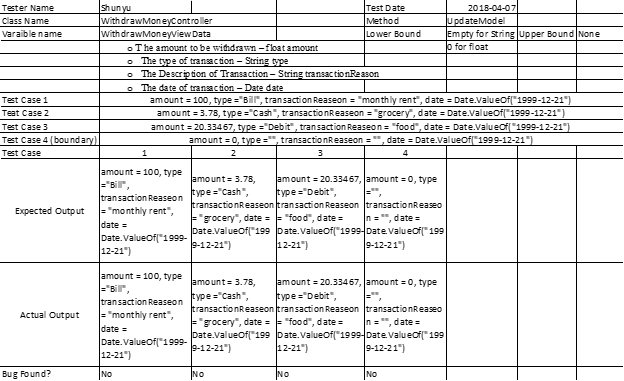
\includegraphics[width=\textwidth]{unit_test_deposit.png}
  \caption{Unit test for Deposit Money use case}
\end{figure}

\subsubsection{Unit Test for Withdraw Money Use Case}

{\bf UpdateModel(WithdrawMoneyViewData data)}\\
Tests will be conducted on UpdateModel method in WithdrawMoneyController Class. Unlike UpdateView, we could only conduct a few unit tests on it since it is a black box and coders can’t not sense whether the model data is updated on the database. So, we have to manually input a series of test data, and verifies whether the real results we read on database are aligned with expected updates. The parameter WithdrawMoneyViewData is a class that contains four field as follows:
\begin{itemize}
  \item The amount to be withdrawn – float amount
  \item The type of transaction – String type
  \item The Description of Transaction – String transactionReason
  \item The date of transaction – Date date
\end{itemize}
When we call UpdateModel taking WithdrawMoneyViewData, it will create a new table row as the first table row, then we read from the first table row and test whether it is the same as the inputs.

\begin{figure}[H]
  \centering
  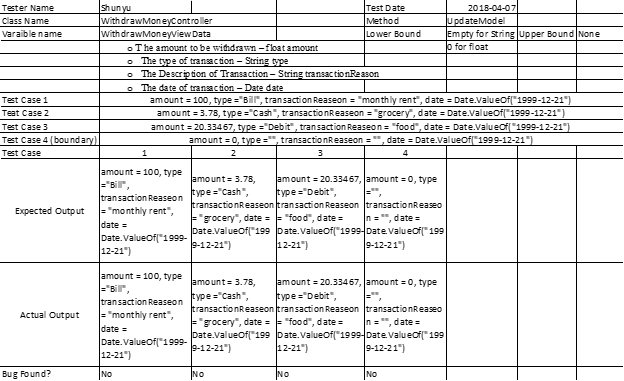
\includegraphics[]{unit_test_withdraw.png}
  \caption{Unit test for Withdraw Money use case}
\end{figure}

\section{Test Results}

In this section we will be outlining the test results for both of our main test cases while providing in depth information regarding regular, special, and boundary cases. 

\subsection{Deposit Money Test}

\subsubsection{Expected Output (when ``Done'' button is clicked, and tests are implemented in order)}

Regular Cases
\begin{itemize}
  \item Value 100: Works as expected.\\
Account: 100.00 Current Balance: 100.00
  \item Value 200.78: Works as expected.\\
Account: 300.78 Current Balance: 300.78
\end{itemize}

Special Cases
\begin{itemize}
  \item Value -50: Does not work as expected. Subtracts 50 from the account and from the ``Current Balance'' field.\\
No error message is displayed.
  \item Value ``Hello'': Works as expected. An error message appears.\\
Error: Value entered must be a positive number.
  \item Value: 3.2222: Works as expected.\\
Account: 304.0022 Current Balance: 304.00
  \item Value -30.55: Subtracts 30.55 from the account and from the ``Current Balance'' field.\\
No error message is displayed.
\end{itemize}

\subsubsection{``Type of Deposit'' input text field}

Boundary Cases
\begin{itemize}
  \item Pass nothing (leave the field empty). Works as expected. The deposit concludes with default reason.
\end{itemize}

Regular Cases
\begin{itemize}
  \item Pass a string  ``Cash Entry''. Works as expected and provides deposit reason.
  \item Pass a string containing a number  ``Money Transfer \#3''. Works as expected and provides deposit reason.
\end{itemize}

\subsubsection{``(optional) Transaction Description'' input text field}

Boundary Cases
\begin{itemize}
  \item Pass nothing (leave the field empty). Works as expected with no description.
\end{itemize}

Regular Cases
\begin{itemize}
  \item Pass a string ``Money found in couch''. Works as expected and provides description.
  \item Pass a string containing a number ``Sold Xbox 360''. Works as expected and provides description.
\end{itemize}

\subsubsection{``Done'' button}

All tests above satisfy this case as they require the use of the Done button. Please refer to sections 1 and 2.
	
\subsubsection{``Cancel'' button}

Regular Cases
\begin{itemize}
  \item Transaction is not recorded. That is:
  \begin{itemize}
    \item Account (database) does not contain a record corresponding to the input. Works as expected.
    \item ``Current Balance field'' is unchanged. Works as expected.
  \end{itemize}
\end{itemize}

\subsection{Withdraw Money Test}

\subsubsection{Expected Output (when ``Done'' button is clicked, and tests are implemented in order)}

Boundary Cases
\begin{itemize}
  \item Passing a 0 or a 0.00: Works as expected, no actual change is done to the balance.
\end{itemize}

Regular Cases
\begin{itemize}
  \item Value of 100: Works as expected, withdrawal is performed.
  \item Value of 200.78: Works as expected. Withdrawal is performed.
\end{itemize}

Special Cases
\begin{itemize}
  \item Value of -50: Does not work as expected.  It adds 50 to the account and to the ``Current Balance'' field. No error message is shown.
  \item Value ``Hello'': Works as expected. An error message is shown.
  \item Value 3.2222: Works as expected by being rounded to the nearest hundredth when performing the withdrawal. 
\end{itemize}

\subsubsection{Expected Output (when ``Show History'' is clicked).}

Boundary Cases
\begin{itemize}
  \item ``'' is under the ``TYPE OF WITHDRAW'': Works as expected. It is left blank.
\end{itemize}

Regular Cases
\begin{itemize}
  \item ``bill'' is under the ``TYPE OF WITHDRAW'': Works as expected. Bill is shown as the type of the withdrawal.
  \item ``check'' is under the ``TYPE OF WITHDRAW'': Works as expected. Check is shown as the type of the withdrawal.
\end{itemize}

\subsubsection{(optional) ``Transaction Description'' input text field.}

Boundary Cases
\begin{itemize}
  \item ``'' is under the ``DESCRIPTION'': Works as expected. It is left blank.
\end{itemize}

Regular Cases
\begin{itemize}
  \item  ``Pay electricity bill of June'' is under the ``DESCRIPTION'': Works as expected. Shows this as the description for the withdrawal.
  \item  ``Pay off the debt owed to Jack'' is under the ``DESCRIPTION'': Works as expected. Shows this as the description for the withdrawal.
\end{itemize}

\subsubsection{``Done'' button}

Expected output is relative to the outlined uses in the above cases. They all require the use of the ``Done'' button, therefore this button is tested through those same tests.
	
\subsubsection{``Cancel'' button}

Regular Cases
\begin{itemize}
  \item Transaction is not recorded. That is:
  \begin{itemize}
    \item Account (database) does not contain a record corresponding to input data: Works as expected.
    \item ``Current Balance'' field is unchanged: Works as expected. No changes occur.
  \end{itemize}
\end{itemize}

\section{References}
We obtained a test document sample that we used as a reference: Montrealopoly, Master Test Plan, from: https://users.encs.concordia.ca/~paquet/wiki/images/3/35/Phase3final.pdf

\appendix

\section{Description of Input Files}

\subsection{Mymoneyappdb.db}

\subsubsection{File Description}
Database file used for SQLite. Contains all the database information locally, such as the different tables and their contents. It contains the following four Tables:
\begin{itemize}
  \item Withdraw\_Money
  \item Deposit\_money
  \item Display\_Balance
  \item sqlite\_sequence
\end{itemize}

\subsubsection{Input Description}
The application will read from this file every time it is run to get all the Database information and display them on the GUI.

\subsection{Transaction\_History.csv}

\subsubsection{File Description}
Excel file used to keep a history of all transactions executed within the application, as well as all the information relating to those transactions. It contains the following six columns:
\begin{itemize}
  \item Date
  \item Transaction Type
  \item Description
  \item Amount
  \item Type of Withdrawal
  \item Type of Deposit
\end{itemize}

\subsubsection{Output Description}
The application will read from this file every time it tries to access the history of all transactions to be able to display them on the GUI.

\section{Description of Output Files}

\subsection{Mymoneyappdb.db}

\subsubsection{File Description}
Database file used for SQLite. Contains all the database information locally, such as the different tables and their contents. It contains the following four Tables:
\begin{itemize}
  \item Withdraw\_Money
  \item Deposit\_money
  \item Display\_Balance
  \item sqlite\_sequence
\end{itemize}

\subsubsection{Output Description}
Everytime a new withdraw or deposit action happens, the application will write to this file to add new entries under their respective tables.  

\subsection{Transaction\_History.csv}

\subsubsection{File Description}
Everytime a new withdraw or deposit action happens, the application will write to this file to add new entries under their respective tables.  
\begin{itemize}
  \item Date
  \item Transaction Type
  \item Description
  \item Amount
  \item Type of Withdrawal
  \item Type of Deposit
\end{itemize}

\subsubsection{Output Description}
Everytime a new withdraw or deposit action happens, the application will write to this file to add new rows containing all the information of the transaction.

\clearpage 
\section{Figures}

\begin{figure}[H]
  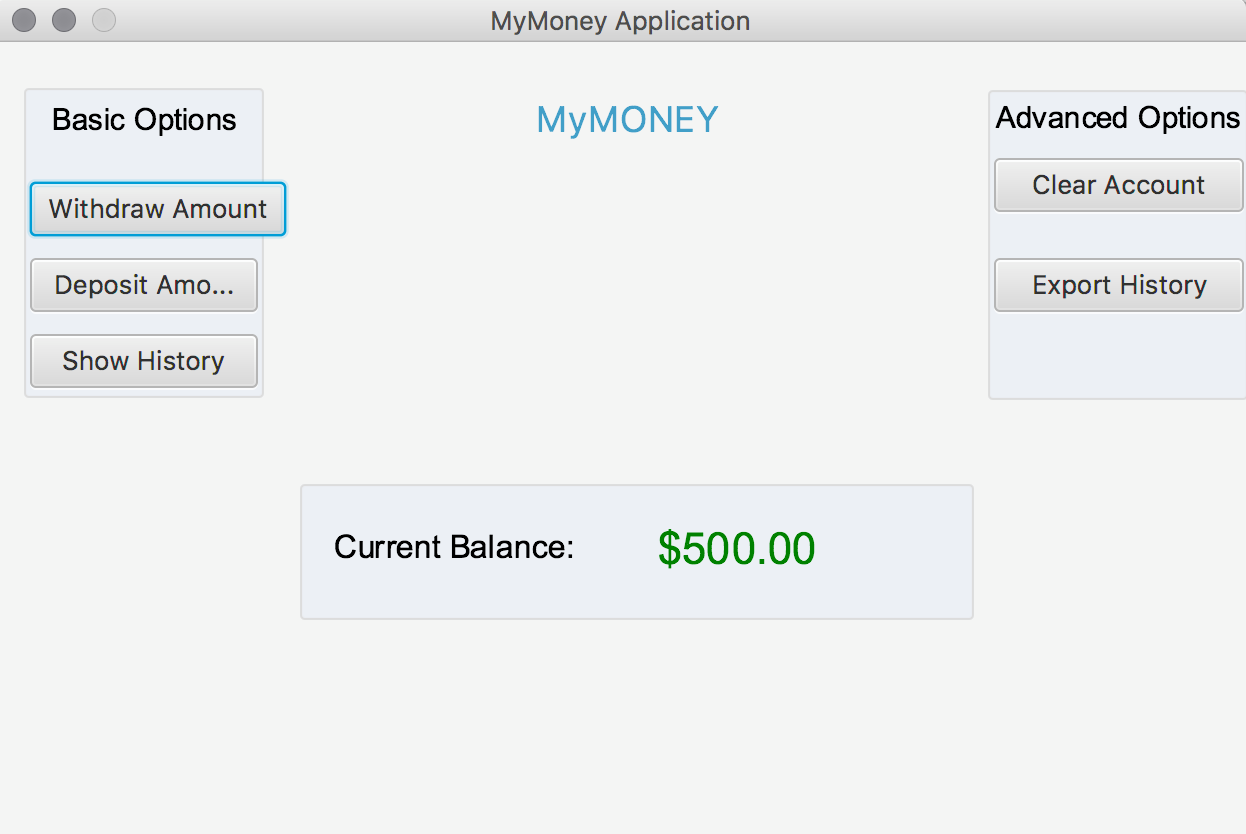
\includegraphics[width=\linewidth]{open_app.png}
  \caption{The user opens myMoney App.}
\end{figure}

\begin{figure}[H]
  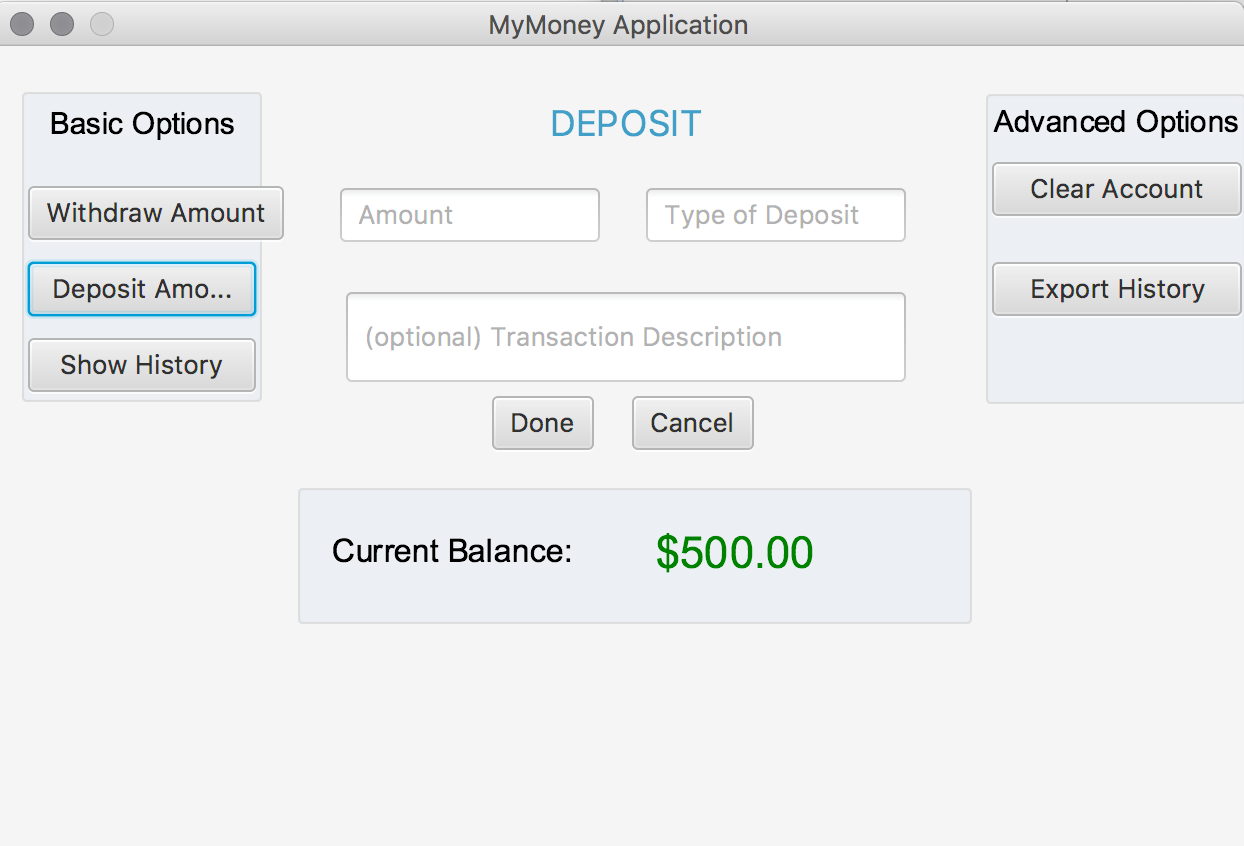
\includegraphics[width=\linewidth]{deposit_click.png}
  \caption{The fields mentioned in the Deposit Test Case section are shown above.}
\end{figure}

\end{document}
